\subsection{Opsætning af server}
Dette afsnit har til formål at beskrive hvordan et udviklingsmiljø sættes op på en givet maskine, så vider udvikling af systemet kan finde sted. Afsnittet forklarer også hvilke tredjeparts teknologier der er anvendt og eventuelle afhængigheder.

\subsubsection*{OS}
Det anbefales at udviklingen finder sted på en OS X eller Linux maskine, da UNIX-terminalen er et meget brugt værktøj og som standart er windows cmd meget "begrænset". Det kan dog lade sig gøre at bruge windows's cmd med nogle tweaks. Dette er ikke noget der vil blive forklaret yderligere og derfor er det kun UNIX-terminalen der er beskrevet i afsnittet.

\subsubsection*{IDE/Text Editor}
Da alt server opsætningen og logikken er skrevet i python, som er et højniveau script sprog, er der ikke nogle specielle krav til et IDE. Et simpelt tekst redigerings program er at fortrække. Det anbefales enten at bruge Sublime\footnote{http://www.sublimetext.com/2} Text Editoren eller Atom\footnote{https://atom.io/} Editoren. Begge text editors tilbyder god code highlightning og mulighed for at tilføje tredje parts pakker. Et udkast af de pakker der bruges er "PyLinter", "pep8" eller "Linter", som tjekker koden for evt. fejl i indentering, manglende kommentar eller kode standart.

\subsubsection*{Installation af software}
Dette underafsnit vil forklare hvordan diverse software pakker installeres på udviklingernes maskine og hvordan udviklerne starter den lokale server op. \\
Det første program der skal installeres er git. Skriv følgende i terminalen.

Linux:
\begin{lstlisting}[language=bash]
	$ sudo apt-get install Git
\end{lstlisting}

\textit{OS X: Kommer som standart med git installeret.}

Efter git er installeret på maskinen skal source koden klones fra github. Skriv følgende i terminalen.

\begin{lstlisting}[language=bash]
	$ git clone https://github.com/Opstrup/drone_backend
\end{lstlisting}

Efter source koden er hentet skal package manager programmet pip\footnote{https://pypi.python.org/pypi/pip} installeres. Skriv følgende i terminalen.

Linux:
\begin{lstlisting}[language=bash]
	$ sudo apt-get install python-pip
\end{lstlisting}

OS X:
\begin{lstlisting}[language=bash]
	$ sudo easy_install pip
\end{lstlisting}

Når pip er installeret skal scriptet "requirements.txt" køres, dette script ligger i roden af server projektet som blev hentet fra github. Skriv følgende i terminalen (da pip bliver brugt som package manager er kommandoen ens på Linux og OS X). \\

\begin{lstlisting}[language=bash]
	$ pip install -r requirements.txt
\end{lstlisting}

Efter scriptet er kørt og pip har installeret alle afhængigheder, er serveren klar til blive startet. For at starte serveren, skriv følgende i terminalen.

\begin{lstlisting}[language=bash]
	$ cd drone_backend_api/
	$ ./manage.py runserver
\end{lstlisting}


På figur \ref{fig:server_startup} ses et udklip af terminal vinduet ved server startup. Det ses at serveren er startet på "http://127.0.0.1:8000/", bemærk at denne url ikke bruges og vil derfor vise en: 404 error page not found fejl, hvis den tilgås. For at tilgå servere kan api endpoints, som beskrevet i Data view afsnittet, benyttes, http://127.0.0.1:8000/api/drones/.
\begin{figure}[H]
	\centering
	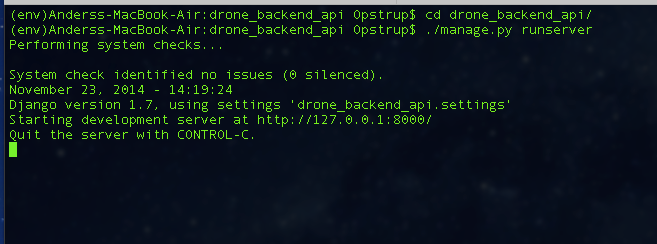
\includegraphics[width=0.85\textwidth]{Billeder/implementation/server_startup.png}
	\caption{Server startup msg}
	\label{fig:server_startup}
\end{figure}
\newpage

\subsubsection*{Mappestruktur}
Dette underafsnit vil forklare om den overordnede mappestruktur i projektet og giver en overordnet forståelse af django udvikling. \\

På figur \ref{fig:mappestruktur_1} ses den overordnet mappestruktur. I roden af mappen findes to væsentlige filer: db.sqlite3 hvilket er database filen til serveren, denne fil vil aldrig blive brugt direkte, men kun indirekte igennem django-frameworket. Den anden fil er manage.py, denne fil er main filen i hele projektet. Filen redigeres aldrig, men bruges kun via terminalen, til forskellige kommandoer på django-applikationen. \\

I roden findes der også to mapper "backend\_api" og "drone\_backend\_api". "drone\_backend\_api"  mappen er selve projekt mappen og "backend\_api" er applikations mappen.

\begin{figure}[H]
	\centering
	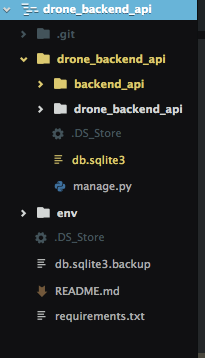
\includegraphics[width=0.2\textwidth]{Billeder/implementation/mappestruktur_1.png}
	\caption{Mappestruktur rod}
	\label{fig:mappestruktur_1}
\end{figure}

På figur \ref{fig:mappestruktur_2} ses projekt mappen, de væsentlige filer i denne mappe er settings.py og urls.py.
Settings.py er filen hvor alle tredje parts applikationer registeres i "INSTALLED\_APPS", filens sikkerhedsindstillinger  sættes op i "MIDDLEWARE\_CLASSES". 
Urls.py filen bruges til at registrere hvilke url's serveren kender og hvilke funktioner og views der skal præsenteres. Yderligere dokumentation omkring settings.py og urls.py kan findes under djangos egen dokumentation omkring settings\footnote{https://docs.djangoproject.com/en/dev/ref/settings/} og urls\footnote{https://docs.djangoproject.com/en/dev/ref/urls/}.

\begin{figure}[H]
	\centering
	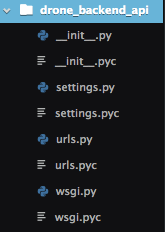
\includegraphics[width=0.2\textwidth]{Billeder/implementation/mappestruktur_2.png}
	\caption{Mappestruktur projekt mappe}
	\label{fig:mappestruktur_2}
\end{figure}

\newpage

På figur \ref{fig:mappestruktur_3} ses applikations mappen. Denne mappe indeholder alt logikken til serveren.

\begin{figure}[H]
	\centering
	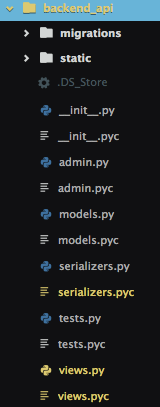
\includegraphics[width=0.2\textwidth]{Billeder/implementation/mappestruktur_3.png}
	\caption{Mappestruktur applikations mappe}
	\label{fig:mappestruktur_3}
\end{figure}

\textbf{admin.py} \\
Denne fil indeholder registrering af diverse tables i projektet. De kan tilgås via en admin page, hvor en administrator kan redigere i det data der ligger i databasen. Yderligere dokumentation omkring admin.py kan findes på\footnote{https://docs.djangoproject.com/en/dev/ref/contrib/admin/}.

\textbf{models.py} \\
Denne fil indeholder alt logikken til hvilke tabeller og attributter der eksistere i databasen. Via denne fil bliver db.sqlite3 filen som findes i roden, manipuleret. Yderligere dokumentation omkring models.py kan findes på\footnote{https://docs.djangoproject.com/en/dev/topics/db/models/}.

\textbf{serializers.py} \\
Denne fil indeholder serializers kaldes når et api-endpoint bliver kaldt. Via disse serializers finder serveren ud af hvilke data der skal hentes fra databasen og repræsenteres. Disse serializers bliver hovedsageligt brugt til at formatere dataen fra databasen til et JSON format. Yderligere dokumentation omkring serializers.py kan findes på\footnote{https://docs.djangoproject.com/en/dev/topics/serialization/}.

\textbf{views.py} \\
Denne fil håndtere de requests som kaldes og afgør ud fra dem hvilke serializer der skal generes og præsenteres. Yderligere dokumentation omkring views.py kan findes på\footnote{https://docs.djangoproject.com/en/dev/topics/class-based-views/}.
\newpage

\subsubsection*{Debug}
Dette underafsnit vil beskrive hvordan server software kan debugges og hvordan de forskellige værktøjer kan bruges.\\

\textbf{Terminal}\\
På figur \ref{fig:get_eksempel} ses et udklip af terminal vinduet, hvor to GET requests har fundet sted. Som det ses på billedet, er det muligt at debugge serveren og tjekke hvilke data sendes frem og tilbage ved hvert request. 

\begin{figure}[H]
	\centering
	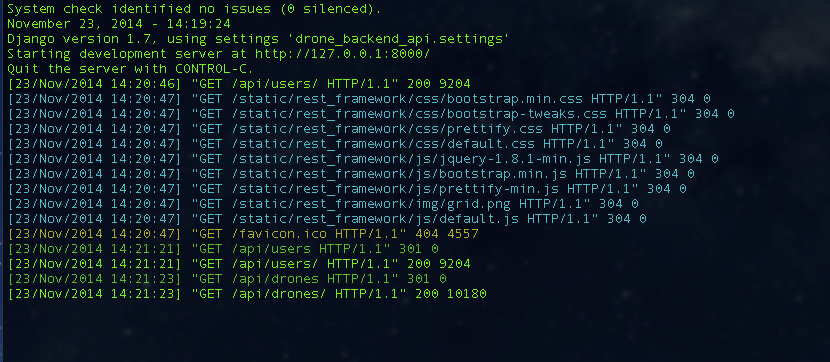
\includegraphics[width=1\textwidth]{Billeder/implementation/get_eksempel.png}
	\caption{GET eksempel}
	\label{fig:get_eksempel}
\end{figure}

\textbf{Browser}\\
På figur \ref{fig:browser_eksempel} ses et andet eksempel på hvordan browseren kan bruges til at debugge serveren. Her ses det hvilke data der kan hentes ved at gå til api-endpoint\\
"http://127.0.0.1:8000/api/drones/". Yderligere information kan findes under Data View afsnittet.

\begin{figure}[H]
	\centering
	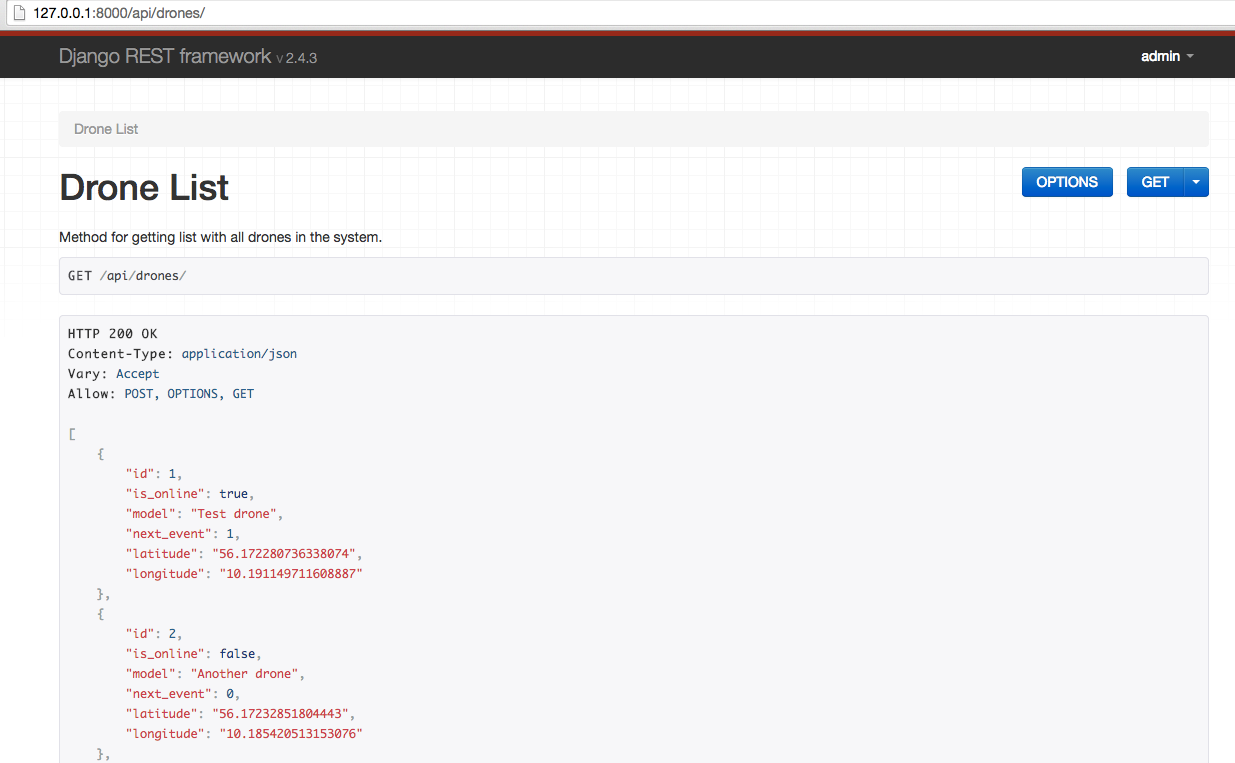
\includegraphics[width=1\textwidth]{Billeder/implementation/browser_eksempel.png}
	\caption{Browser eksempel}
	\label{fig:browser_eksempel}
\end{figure}

\vspace{1cm}

\subsubsection*{Tredje parts teknologier}
Til udviklingen af server softwaren er der benyttet nogle tredje parts teknologier, dette underafsnit beskriver hvilke og hvordan de er blevet brugt.

\textbf{Djangorestframework}\\
Django frameworket er et godt framework til udvikling af webapplikationer.Til projektet ønskes et RESTful api oven på django frameworket, derfor er der brugt et django-rest-frameworket\footnote{http://www.django-rest-framework.org/}. 

\textbf{django-cors-headers}\\
Cors headers\footnote{https://github.com/ottoyiu/django-cors-headers} er et django applikation som tilføjer CORS (Cross-Origin Resource Sharing) til applikationer. Dette gør det muligt at tilgå applikationen fra andre servere, som fx.  client softwaren som kan ligge på en anden server eller dronen som tilgår serveren udefra. 

\newpage